\chapter{Anhang}

\section{Lösungen zu Kapitel 1}

Hier findest du die Lösungen zur Selbstkontrolle!


\begin{Loesung}[zu Aufgabe \ref{Aufg:Strom}] \label{Loes:Strom}
\emph{Elektrischer Strom} ist die Bewegung von \emph{elektrischen Ladungsträgern} (zB. Elektronen) in eine gemeinsame Richtung.

Dieser ist nur in  geschlossenen Kreisläufen möglich, man spricht vom \emph{elektrischen Stromkreis}.

Die Bewegung der Ladungsträger wird von einer \emph{Spannungsquelle} hervorgerufen.
\end{Loesung}


\begin{Loesung}[zu Aufgabe \ref{Aufg:Kirchhoff1} und \ref{Aufg:Kirchhoff2}]
Die vollständigen Werte:
\begin{center}
\includegraphics[scale=.65]{pics/Kirchhoffloes}
\end{center}

\end{Loesung}


\section{Lösungen zu Kapitel 2}

\begin{Loesung}[zu Aufgabe \ref{Aufg:SensorSimul}]
Oben (a), unten (b)
\begin{center}
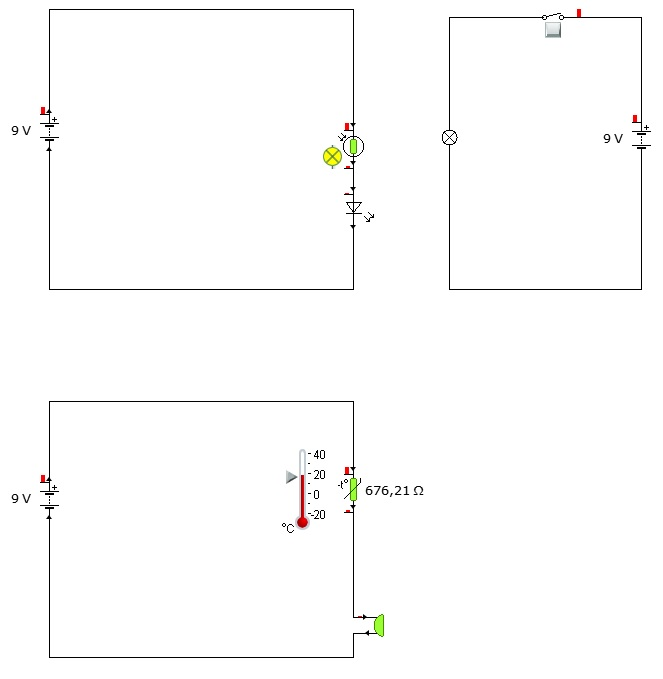
\includegraphics[width=.7\textwidth]{pics/loessimu}
\end{center}
\end{Loesung}



\begin{Loesung}[zu Aufgabe \ref{Aufg:DiodeTest}]
\hfill \par \vspace*{-.7cm}
\begin{itemize}
\item[(a)] 
\begin{tabular}{|c|c|c|c|c|c|c|c|c|c|}
\hline
$U$ in V & 0,1 & 0,2 & 0,3 & 0,4 & 0,5 & 0,6 & 0,7 & 0,8 & 0,9 \\ \hline
$I$ & 0,01 & 0,01 & 0,02 & 0,17 & 8,39 & 393 & 20 mA & 987 mA & z \\ \hline
\end{tabular}
\item[(b)] 
\begin{tabular}{|c|c|c|c|c|c|c|}
\hline
$U$ in V & 0,5 & 1 & 10 & 25 & 50 & 51  \\ \hline
$I$ &0&0&0&0&0& zerstört \\ \hline
\end{tabular}
\item[(c)] Die Diode kann in zwei Richtungen betrieben werden, in der einen Richtung (a), lässt sie Strom fließen, bis ca. 0,9 $V$, dann wird sie zerstört.
In der anderen Richtung lässt sie keinen Stromfluss zu, bis ca. 51 $V$, dann wird sie zerstört.
\end{itemize}

\end{Loesung}




\begin{Loesung}[zu Aufgabe \ref{Aufg:Diodenlogik}]
Die Lösung:
\begin{center}
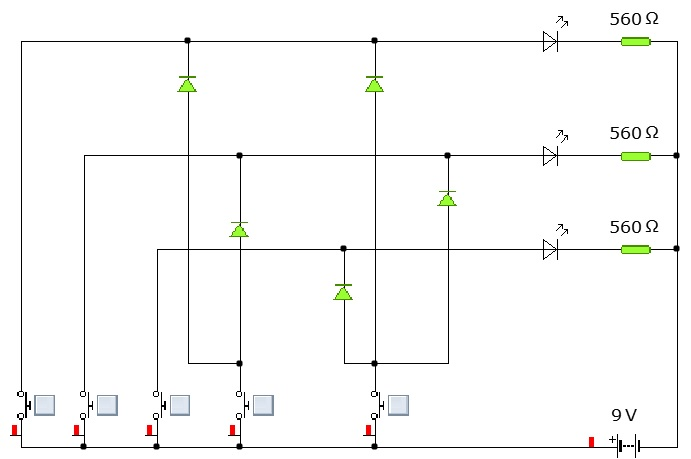
\includegraphics[scale=.6]{pics/loesdiodenlogik}
\end{center}
\end{Loesung}




\begin{Loesung}[zu Aufgabe \ref{Aufg:Inverter}]
\hfill \par
\begin{center}
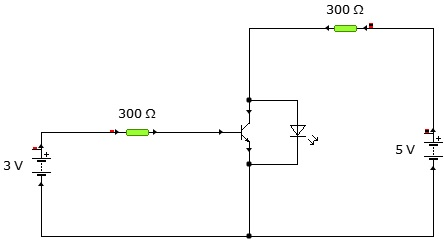
\includegraphics[scale=.6]{pics/NegatorLoes}
\end{center}

Die LED (bzw. der Ausgang) muss parallel zum Transistor geschaltet werden. Wird die Basis mit niedriger Spannung angesteuert (0) dann wird der Widerstand des Transistors sehr groß und der Strom der Kollektor-Emitter-Strecke fließt über die LED ab (Ausgang 1).

Wird die Basis mit hoher Spannung angesteuert (1), dann wird der Widerstand des Transistors klein (und kleiner als der Widerstand der LED) und der Strom der Kollektor-Emitter-Strecke fließt über den Transistor ab (Ausgang 0).
\end{Loesung}

\begin{Loesung}[zu Aufgabe \ref{Aufg:Daemmerung}]
\hfill \par
\begin{center}
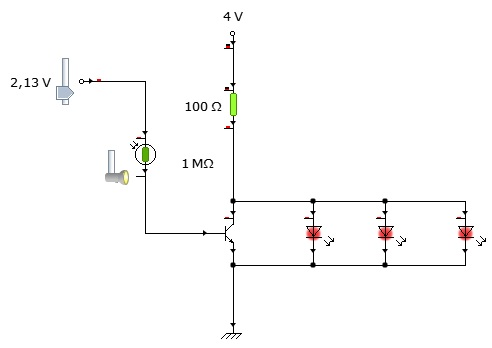
\includegraphics[scale=.8]{pics/Daemmerungeinf}
\end{center}

Die Spannung an der Basis dient als Eingangsspannung.
Die Spannung am Emitter dient als Arbeitsspannung.
Die LEDs sind parallel zum Transistor geschaltet, um deren Arbeitsweise zu invertieren.
\end{Loesung}


\begin{Loesung}[zu Aufgabe \ref{Aufg:TransistorKomplex}]
\hfill \par
\begin{center}
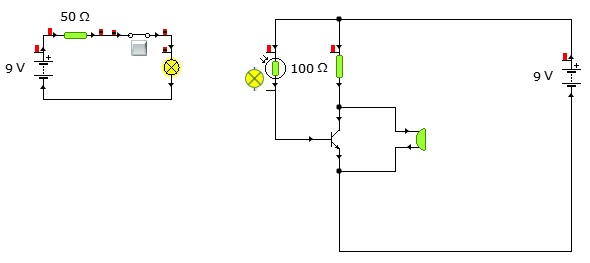
\includegraphics[scale=.8]{pics/TransistorKomplexN1}
\end{center}

\begin{itemize}
\item[(N1)] Die Schaltung links dient als Steuerschaltung für den Fotowiderstand im Arbeitsstromkreis (rechts). Der Buzzer ist parallel zum Transistor geschaltet, um seine Eigenschaften zu invertieren.
\end{itemize}

\begin{center}
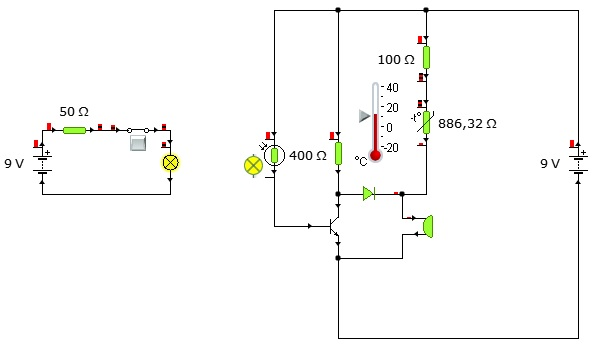
\includegraphics[scale=.8]{pics/TransistorKomplexN2}
\end{center}

\begin{itemize}
\item[(N2)] Der Thermistor steuert den Buzzer direkt an, da in diesem Fall die Eigenschaften nicht invertiert werden sollen. Damit der Thermistorstrom nicht über den Transistor abfließen kann, ist auf der entsprechenden Leitung unbedingt eine Diode einzufügen, die den Stromfluss nur in die andere Richtung zulässt!
\end{itemize}

\begin{center}
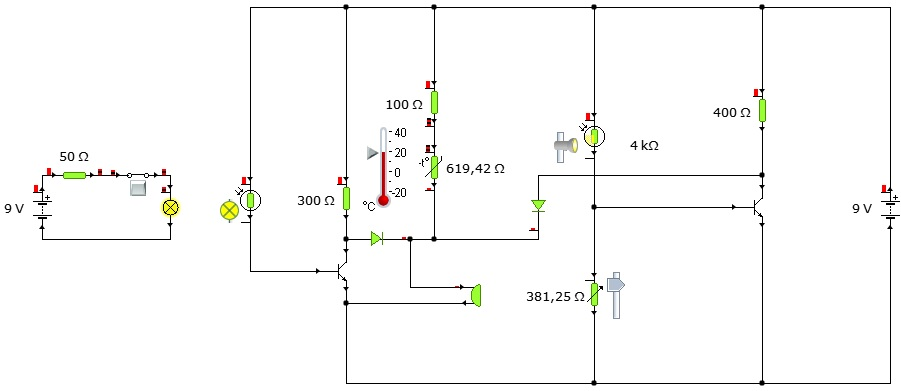
\includegraphics[scale=.7]{pics/TransistorKomplexN3}
\end{center}

\begin{itemize}
\item[(N3)] 
\end{itemize}

\end{Loesung}


\begin{Loesung}[zu Aufgabe \ref{Aufg:SchmittTest}]

Der Schmitt-Inverter dient als Schwellenwertschalter. Bis zu einer gewissen Schwellspannung gibt er am Ausgang log. 1 aus. Nach dieser Schwellspannung gibt er am Ausgang log. 0 aus.
\end{Loesung}